% Build:
%   latexmk -pdf -interaction=nonstopmode -halt-on-error -outdir=docs/.build docs/vivatech-pwc-dossier-technique-praedixa-2026.tex
% Output PDF:
%   docs/.build/vivatech-pwc-dossier-technique-praedixa-2026.pdf
\documentclass[11pt,a4paper]{article}

\usepackage[a4paper,margin=22mm]{geometry}
\usepackage[T1]{fontenc}
\usepackage[utf8]{inputenc}
\usepackage{lmodern}
\usepackage{microtype}
\usepackage{hyperref}
\usepackage{enumitem}
\usepackage{titlesec}
\usepackage{graphicx}
\usepackage{xcolor}
\usepackage{booktabs}
\usepackage{tabularx}
\usepackage{tikz}
\usetikzlibrary{arrows.meta,positioning,shapes.geometric,fit}

\definecolor{PraedixaBlue}{HTML}{0B4F6C}
\definecolor{PraedixaTeal}{HTML}{01BA9A}
\definecolor{PraedixaGray}{HTML}{2B2D42}
\definecolor{PraedixaLight}{HTML}{F4F6F8}

\hypersetup{
  colorlinks=true,
  linkcolor=PraedixaBlue,
  urlcolor=PraedixaBlue
}

\setlist[itemize]{leftmargin=*,nosep}
\titleformat{\section}{\large\bfseries\color{PraedixaGray}}{}{0em}{}
\titleformat{\subsection}{\normalsize\bfseries\color{PraedixaGray}}{}{0em}{}

\newcommand{\pill}[1]{\colorbox{PraedixaLight}{\strut\hspace{0.4em}\textsf{\small #1}\hspace{0.4em}}}

\begin{document}

\begin{center}
  {\LARGE \textbf{Praedixa} \par}
  \vspace{2mm}
  {\large Dossier technique (VivaTech x PwC - Etudiants 2026) \par}
  \vspace{2mm}
  {\small Version: \today \par}
  \vspace{4mm}
  \pill{Ops/DAF} \hspace{2mm}
  \pill{J+3 / J+7 / J+14} \hspace{2mm}
  \pill{Scenarios cout vs service} \hspace{2mm}
  \pill{Proof / audit-ready}
\end{center}

\vspace{4mm}

\section*{1. Resume executif}
Praedixa est une couche de pilotage \textbf{Ops/DAF} au-dessus des outils existants (WFM/ERP/tableurs) qui:
\begin{itemize}
  \item \textbf{anticipe} les risques de rupture de couverture a \textbf{J+3/J+7/J+14},
  \item \textbf{explique} les drivers actionnables (absences, charge, contraintes),
  \item \textbf{chiffre} l'arbitrage \textbf{cout vs service} via des scenarios (HS, interim, reallocation, ajustement de service),
  \item \textbf{prouve} l'impact via un protocole de mesure (0\% / 100\% / reel) et un decision log.
\end{itemize}
Notre difference: ce n'est pas un dashboard, ni une ``prediction IA'' decorative; c'est un systeme \textbf{audit-ready} (hypotheses explicites, versioning, tracabilite, rejouabilite).

\section*{2. Contexte et probleme}
Dans les operations multi-sites a forte intensite de main-d'oeuvre (logistique, industrie, retail, sante), les decisions de capacite sont souvent prises trop tard (J-0/J-1) a cause de:
\begin{itemize}
  \item donnees eclatees et definitions non alignees (activite, capacite/couverture, absences, couts),
  \item contraintes terrain difficiles a formaliser (caps HS, lead time interim, polyvalence),
  \item arbitrages implicites et non comparables (HS vs interim vs reallocation vs service degrade),
  \item absence de preuve defendable pour la DAF (attribution des gains, justification a posteriori).
\end{itemize}

\section*{3. Proposition de valeur (comment on cree de la valeur)}
\begin{itemize}
  \item \textbf{Decider plus tot}: transformer J-0/J-1 en J+3/J+7/J+14 pour activer des options moins cheres et plus faisables.
  \item \textbf{Comparer des options reelles}: generer des scenarios avec cout total attendu, service attendu, faisabilite, sous contraintes explicites.
  \item \textbf{Rendre l'arbitrage audit-ready}: decision log + hypothese versionnee + preuve reguliere (proof pack).
  \item \textbf{Demarrer vite}: exploitation d'exports agreges, sans projet SI lourd, privacy-by-design.
\end{itemize}

\section*{4. Technologie et architecture (vue d'ensemble)}
\subsection*{4.1 Stack logicielle}
\begin{itemize}
  \item \textbf{Frontend (dashboard client / back-office)}: Next.js 15, React 19, Tailwind CSS. Deploiement possible sur Cloudflare Workers via OpenNext.
  \item \textbf{Backend API}: FastAPI (Python), SQLAlchemy 2 async, PostgreSQL 16, Alembic, Pydantic 2, JWT (Supabase JWKS).
  \item \textbf{Securite et isolation}: multi-tenancy (TenantFilter + SiteFilter) et RLS PostgreSQL, rate limiting (slowapi), CSP nonce.
  \item \textbf{Data engineering}: pipeline ``medallion'' bronze -> silver -> gold (metadata-driven), anti-leakage temporel.
  \item \textbf{Livrable preuve}: generation de rapports / proof packs (PDF) a partir de donnees versionnees.
\end{itemize}

\subsection*{4.2 Diagramme d'architecture}
\begin{center}
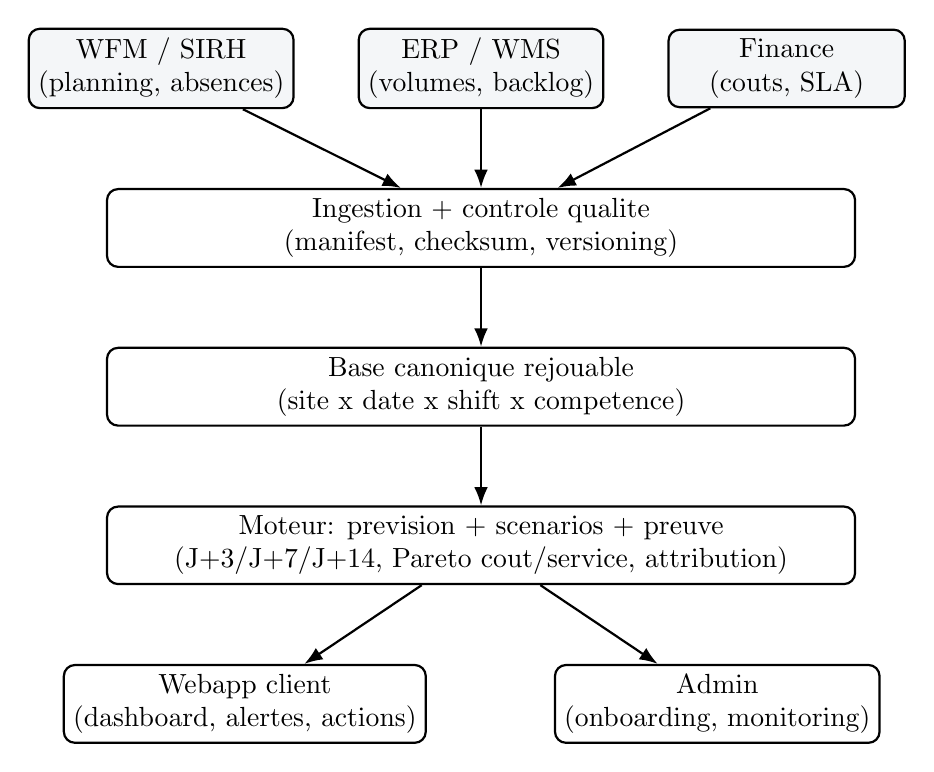
\begin{tikzpicture}[
  node distance=10mm,
  box/.style={draw, rounded corners, thick, align=center, minimum width=30mm, minimum height=9mm},
  src/.style={box, fill=PraedixaLight},
  svc/.style={box, fill=white},
  arr/.style={-Latex, thick}
]
  \node[src] (wfm) {WFM / SIRH\\(planning, absences)};
  \node[src, right=8mm of wfm] (erp) {ERP / WMS\\(volumes, backlog)};
  \node[src, right=8mm of erp] (cost) {Finance\\(couts, SLA)};

  \node[svc, below=10mm of erp, minimum width=95mm] (ingest) {Ingestion + controle qualite\\(manifest, checksum, versioning)};
  \node[svc, below=10mm of ingest, minimum width=95mm] (canon) {Base canonique rejouable\\(site x date x shift x competence)};
  \node[svc, below=10mm of canon, minimum width=95mm] (engine) {Moteur: prevision + scenarios + preuve\\(J+3/J+7/J+14, Pareto cout/service, attribution)};

  \node[svc, below=10mm of engine, xshift=-30mm] (webapp) {Webapp client\\(dashboard, alertes, actions)};
  \node[svc, below=10mm of engine, xshift=30mm] (admin) {Admin\\(onboarding, monitoring)};

  \draw[arr] (wfm) -- (ingest);
  \draw[arr] (erp) -- (ingest);
  \draw[arr] (cost) -- (ingest);
  \draw[arr] (ingest) -- (canon);
  \draw[arr] (canon) -- (engine);
  \draw[arr] (engine) -- (webapp);
  \draw[arr] (engine) -- (admin);
\end{tikzpicture}
\end{center}

\section*{5. Data engineering: ``canonique'' + pipeline medaillon}
\subsection*{5.1 Principe}
Praedixa commence par construire une \textbf{source unique rejouable} ``charge-capacite-cout'' a granularite operationnelle:
\begin{itemize}
  \item Grain cible: \textbf{site x date x shift x competence} (competence optionnelle en MVP).
  \item Objectif: fiabilite, fraicheur quotidienne, et tracabilite (mapping source -> canonique versionne).
  \item Mode degrade: si donnees insuffisantes, on prefere un \textbf{rapport de qualite} plutot qu'une recommandation hasardeuse.
\end{itemize}

\subsection*{5.2 Bronze -> Silver -> Gold (anti-leakage)}
\begin{center}
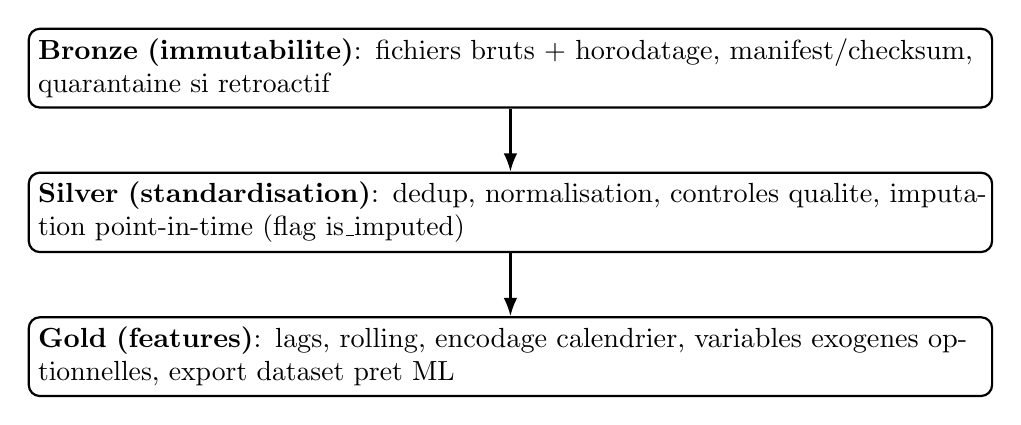
\begin{tikzpicture}[
  node distance=8mm,
  pstep/.style={draw, rounded corners, thick, align=left, text width=120mm, minimum height=10mm},
  arr/.style={-Latex, thick}
]
  \node[pstep] (b) {\textbf{Bronze (immutabilite)}: fichiers bruts + horodatage, manifest/checksum, quarantaine si retroactif};
  \node[pstep, below=of b] (s) {\textbf{Silver (standardisation)}: dedup, normalisation, controles qualite, imputation point-in-time (flag is\_imputed)};
  \node[pstep, below=of s] (g) {\textbf{Gold (features)}: lags, rolling, encodage calendrier, variables exogenes optionnelles, export dataset pret ML};
  \draw[arr] (b) -- (s);
  \draw[arr] (s) -- (g);
\end{tikzpicture}
\end{center}

\subsection*{5.3 Quality gates, SLO, et versioning}
La base canonique et les calculs sont \textbf{versionnes} (mapping, parametres de cout, regles de transformation). Les garde-fous reduisent les faux positifs et evitent les recommandations ``fragiles'':
\begin{itemize}
  \item \textbf{Fraicheur}: refresh quotidien, avec indicateur de ``data staleness'' si J-1 n'est pas disponible.
  \item \textbf{Completude}: si trop de creneaux manquants (charge ou couverture), passage en mode ``data gap report''.
  \item \textbf{Tracabilite}: chaque alerte et scenario est reliable aux lignes canoniques et a la version des regles.
  \item \textbf{Rejouabilite}: rejouer 12-24 mois d'historique pour backtests et audits.
\end{itemize}

\section*{6. Moteur de decision: prevision + scenarios cout/service}
\subsection*{6.1 Prevision orientee decision}
L'objectif n'est pas de predire un volume ``moyen'', mais de predire un \textbf{risque de sous-couverture} (probabilite + severite) par site et par creneau a J+3/J+7/J+14, avec:
\begin{itemize}
  \item calibration des probabilites (reduction du bruit),
  \item explication des drivers (interpretabilite),
  \item garde-fous (pas de recommandation si la data est trop incomplete).
\end{itemize}

\subsection*{6.2 Scenarios et Pareto cout/service}
Pour chaque alerte critique, Praedixa genere un espace d'actions:
\begin{itemize}
  \item options typiques: HS, interim, reallocation intra/inter-sites, ajustement de service (backlog accepte), sous-traitance;
  \item evaluation: \textbf{cout total attendu}, service attendu, faisabilite (lead time, caps, disponibilites);
  \item sortie: frontiere \textbf{non dominee} (Pareto) + recommandation parametrable (ex: cout minimal sous service >= seuil).
\end{itemize}

\subsection*{6.3 Modeles possibles (du baseline au deep learning)}
Le systeme est concu pour supporter plusieurs families de modeles, selectionnees selon volume de donnees, stabilite, besoin d'explicabilite, et cout d'exploitation:
\begin{itemize}
  \item \textbf{Baselines rapides}: Prophet (tendance + saisonnalites), SARIMAX (ARIMA saisonnier + variables exogenes).
  \item \textbf{ML tabulaire (souvent meilleur compromis)}: XGBoost (ou LightGBM) sur features point-in-time (lags, rolling, calendrier, signaux exogenes).
  \item \textbf{Deep learning (gros clients / beaucoup d'historique)}: Temporal Fusion Transformer (TFT), et variantes Transformer / sequence models, pour capter non-linearites et interactions complexes.
  \item \textbf{Ensembles et selection}: comparaisons par backtests, par horizon (J+3/J+7/J+14), et selection du meilleur modele par site/segment si necessaire.
\end{itemize}
Garde-fous indispensables: features strictement \textbf{point-in-time} (anti-leakage), calibration des probabilites, monitoring de drift, et mode degrade si data incompl\u`ete.

\subsection*{6.4 Plug aux agences d'interim (preferred suppliers)}
Objectif: passer de ``je detecte un risque'' a ``je couvre le risque'' en reservant tot une capacite flexible, puis en l'exercant uniquement si necessaire.
\begin{itemize}
  \item \textbf{Principe}: a J+7/J+14, Praedixa envoie des \textbf{pre-reservations} (ou demandes) aux agences referencees, avec une regle d'annulation explicite (ex: annulable T-48).
  \item \textbf{Effet economique}: reserver tot augmente la probabilite d'etre pourvu et reduit le recours au fallback (HS urgence + non-service). On remplace l'urgence par une flexibilite maitrisee.
  \item \textbf{Positionnement}: pas une marketplace; un connecteur d'execution vers un panel de fournisseurs preferes avec KPI/SLA.
\end{itemize}

\subsubsection*{Flux d'execution (pre-reservation -> confirmation -> exercice/annulation)}
\begin{center}
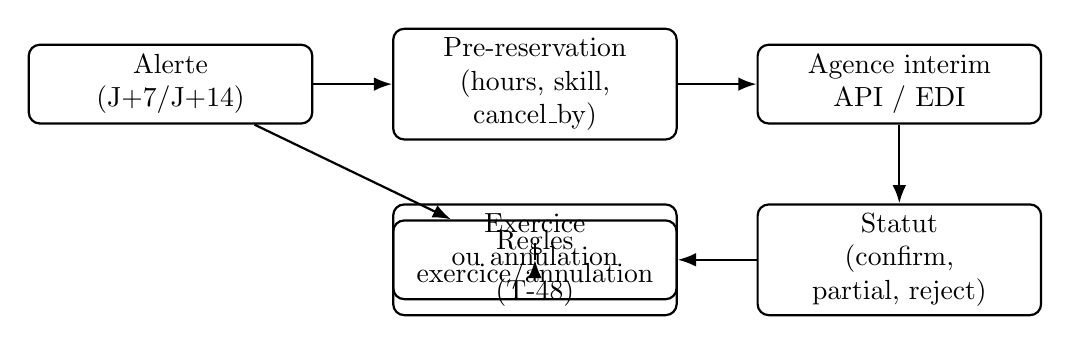
\begin{tikzpicture}[
  node distance=10mm,
  box/.style={draw, rounded corners, thick, align=center, minimum width=36mm, minimum height=10mm},
  arr/.style={-Latex, thick}
]
  \node[box] (risk) {Alerte\\(J+7/J+14)};
  \node[box, right=10mm of risk] (req) {Pre-reservation\\(hours, skill,\\ cancel\_by)};
  \node[box, right=10mm of req] (agency) {Agence interim\\API / EDI};
  \node[box, below=10mm of agency] (status) {Statut\\(confirm,\\ partial, reject)};
  \node[box, below=10mm of req] (rules) {Regles\\exercice/annulation};
  \node[box, left=10mm of status] (exec) {Exercice\\ou annulation\\(T-48)};

  \draw[arr] (risk) -- (req);
  \draw[arr] (req) -- (agency);
  \draw[arr] (agency) -- (status);
  \draw[arr] (status) -- (exec);
  \draw[arr] (rules) -- (exec);
  \draw[arr] (risk) -- (rules);
\end{tikzpicture}
\end{center}

\subsubsection*{Donnees echangees (exemples)}
\begin{itemize}
  \item \textbf{Demande}: site, date, shift, competence (optionnel), heures, priorite, budget (optionnel), \texttt{cancel\_by}, contraintes (badge, horaires, temperature, etc.), idempotency key.
  \item \textbf{Reponse}: confirmation\_id, capacite confirme, taux de remplissage estime, delai, conditions d'annulation, prix (si applicable), raison de rejet.
  \item \textbf{Evenements}: confirmations, modifications, no-show, heures realisees, facturation agregee, afin d'alimenter KPI/SLA et preuve.
\end{itemize}

\subsubsection*{Pourquoi l'agence accepte de se brancher (incentives)}
\begin{itemize}
  \item plus de missions pourvues (visibilite J+7/J+14) => CA en hausse,
  \item cout de sourcing en baisse (moins de mode pompier) => marge en hausse,
  \item stabilite grace aux regles d'ajustement/annulation => moins d'aleas,
  \item KPI/SLA (fill rate, no-show, lead time) => amelioration continue et avantage competitif,
  \item volume recurrent via le statut ``fournisseur prefere''.
\end{itemize}

\subsubsection*{Garde-fous (qualite, securite, et audit)}
\begin{itemize}
  \item \textbf{Tracabilite}: chaque reservation/exercice/annulation est inscrit dans le decision log et relie a une alerte/scenario.
  \item \textbf{Control plane}: quotas par site, caps hebdo, et validation humaine si seuil (cout, volume, service) depasse.
  \item \textbf{Securite}: webhooks signes, idempotence, retries, et separation des secrets; aucun besoin de donnees individuelles pour demarrer (agregats).
  \item \textbf{Mesure}: KPIs (fill rate, lead time, no-show, emergency avoidance, option efficiency) et proof pack (0\%/100\%/reel).
\end{itemize}

\section*{7. Preuve d'impact: decision log + 0\% / 100\% / reel}
\begin{center}
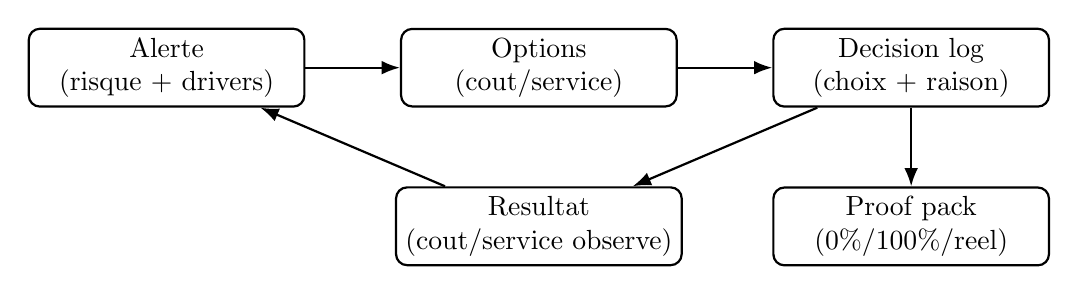
\begin{tikzpicture}[
  node distance=9mm,
  box/.style={draw, rounded corners, thick, align=center, minimum width=35mm, minimum height=9mm},
  arr/.style={-Latex, thick}
]
  \node[box] (alert) {Alerte\\(risque + drivers)};
  \node[box, right=12mm of alert] (options) {Options\\(cout/service)};
  \node[box, right=12mm of options] (decision) {Decision log\\(choix + raison)};
  \node[box, below=10mm of options] (outcome) {Resultat\\(cout/service observe)};
  \node[box, below=10mm of decision] (proof) {Proof pack\\(0\%/100\%/reel)};

  \draw[arr] (alert) -- (options);
  \draw[arr] (options) -- (decision);
  \draw[arr] (decision) -- (proof);
  \draw[arr] (decision) -- (outcome);
  \draw[arr] (outcome) -- (alert);
\end{tikzpicture}
\end{center}
Le protocole de preuve permet d'eviter les effets d'annonce: on compare un scenario ``business-as-usual'' (0\%), un scenario ``application systematique'' (100\%), et le reel.

\section*{8. Securite, conformite, et privacy-by-design}
\begin{itemize}
  \item Donnees agregees par defaut (pas d'individus au depart), minimisation et perimetre defini au cadrage.
  \item Auth JWT via Supabase (JWKS en prod), roles applicatifs, et isolation multi-tenant.
  \item RLS PostgreSQL pour durcir l'isolation a la couche base.
  \item Tracabilite: versioning des regles (mapping, couts) et rejouabilite des calculs.
\end{itemize}

\subsection*{8.1 Multi-tenancy (defense en profondeur)}
\begin{itemize}
  \item \textbf{Couche applicative}: TenantFilter (organization\_id) + SiteFilter (site\_id) sur les queries.
  \item \textbf{Couche base}: RLS PostgreSQL avec variable de session (app.current\_organization\_id) appliquee par transaction.
  \item \textbf{Couche web}: CSP nonce, session verifiee cote serveur, et separation des roles super-admin (back-office).
\end{itemize}

\section*{9. Surface produit: API + ecrans (prototype)}
\subsection*{9.1 API (exemples de modules)}
\begin{tabularx}{\textwidth}{@{}lX@{}}
\toprule
\textbf{Domaine} & \textbf{Ce que ca permet} \\
\midrule
Datasets / Canonical & ingestion fichiers, qualite data, exploration du canonique (charge/capacite) \\
Forecasts / Alerts & runs de prevision, alertes de couverture, priorisation, explication des drivers \\
Scenarios / Arbitrage & generation d'options, evaluation cout/service, frontiere non dominee, overrides \\
Proof & decision log, preuves mensuelles, exports / proof pack PDF \\
\bottomrule
\end{tabularx}

\section*{9. Prototype / demo (etat actuel)}
Un prototype fonctionnel couvre deja les parcours clefs:
\begin{itemize}
  \item dashboard (KPI, previsions 14j, alertes),
  \item page ``actions'' (alertes de couverture, scenarios d'arbitrage),
  \item page ``rapports'' (proof packs, historique, exports),
  \item API documentee (OpenAPI en dev) et back-office super-admin.
\end{itemize}
Objectif demo: montrer un parcours bout-en-bout (donnees -> alerte -> options -> decision -> preuve).

\subsection*{9.2 Scenario de demo (5 minutes)}
\begin{itemize}
  \item Import d'un dataset (planning / absences / volumes) et affichage du rapport qualite.
  \item Visualisation d'une alerte critique a J+7 avec drivers (pourquoi ce site, ce creneau).
  \item Generation de 3 options (HS, interim, reallocation) avec cout/service/faisabilite.
  \item Choix d'une option, ecriture du decision log, puis lecture du proof pack (0\% / 100\% / reel).
\end{itemize}

\section*{10. Comment et pourquoi nous sommes differents}
\subsection*{10.1 Comment (mecanismes concrets)}
\begin{itemize}
  \item \textbf{Boucle complete}: base canonique rejouable -> prevision J+3/J+7/J+14 -> scenarios cout/service -> decision log -> proof pack.
  \item \textbf{Execution (pas juste recommandation)}: plug aux agences d'interim (preferred suppliers) pour pre-reserver, confirmer, exercer/annuler avec regles explicites (T-48).
  \item \textbf{Quality gates + anti-leakage}: pipeline bronze/silver/gold, features strictement point-in-time, calibration, et mode degrade si la data est insuffisante.
  \item \textbf{Interpretable et gouvernable}: drivers par alerte (explain), contraintes explicites (caps, lead time, polyvalence), et parametrage versionne.
  \item \textbf{Defense en profondeur}: multi-tenancy (filtres applicatifs + RLS PostgreSQL) et securite web (CSP, session verifiee cote serveur).
\end{itemize}

\subsection*{10.2 Pourquoi (ce que ca change business)}
\begin{itemize}
  \item \textbf{Moins de mode pompier}: decisions plus tot, moins de HS/interim urgent, et moins de desorganisation.
  \item \textbf{Service stabilise}: reduction des trous critiques et des couts associes (penalites, expedite), avec risque residuel explicite.
  \item \textbf{DAF-ready}: arbitrages defensibles (hypotheses, versioning, tracabilite) et preuve reguliere via 0\% / 100\% / reel.
  \item \textbf{Adoption terrain}: options comparables (cout/service/faisabilite) et regles d'execution simples, reutilisables.
  \item \textbf{Ecosysteme aligne}: incentives agences (fill rate, lead time, stabilite) et selection de fournisseurs preferes sur KPI/SLA.
\end{itemize}

\section*{11. Roadmap (MVP -> premium)}
\begin{itemize}
  \item \textbf{MVP (6-8 semaines)}: canonique stable, alertes J+3/J+7/J+14, 2-3 options principales, decision log v1, proof pack v1.
  \item \textbf{Premium (3-6 mois)}: contraintes avancees (polyvalence, caps hebdo, ramp-up), meilleures features, calibration renforcee, attribution plus robuste.
\end{itemize}

\vspace{2mm}
\noindent \textbf{Contact:} Steven Poivre --- \href{mailto:steven.poivre@outlook.com}{steven.poivre@outlook.com}

\end{document}
